\documentclass[11pt]{article}
\usepackage{icmlko}
\begin{document}

\title{갈래를 한 눈금에 놓다 --- 판은 샀고 전이는 못 샀다, 그래서 설명 하나가 죽는다}
\author{월드모델 실험실}
\date{노트 419 · 2026년 8월 2일}
\maketitle

\begin{abstract}
노트 417·418이 \texttt{grp} 로 안 본 도메인의 전이를 샀다(KR 만화
$-0.0822 \to +0.2128$ · 비게임 앱 $+0.0421 \to +0.1474$). 그때 적은 설명은
\textbf{두 개가 섞여} 있었다 --- ① \emph{grp 가 나르는 성질은 새 작품에도
있어서 안 본 도메인이 낯선 자리에 안 선다}(좌표의 친숙함) ② \emph{grp 가
도메인 사이 분산을 흡수하니 공유 축이 도메인 안에서 일한다}(분산 흡수).
둘을 가르는 시험을 지었다.

레코드 전수조사에서 \texttt{genres} 를 찾았다 --- \textbf{다섯 도메인}
(만화 · 모바일 · 애니 · 세계애니 · 게임)에 $80\%$ 넘게 차 있고 전부 기획
시점 값이다. \texttt{grpaxes} 와 다르게 지었다: 어휘가 실제로 겹치므로
(romance/로맨스 · action/액션 · fantasy/판타지) \textbf{눈금을 도메인
사이에서 공유한다} --- 다섯을 합쳐 세고 그 순위를 모두가 같이 쓴다.

\textbf{결정적으로 gen 은 안 본 도메인에도 값이 있다.} KR 만화 1{,}716건 중
\textbf{1{,}713건}을 채웠다. grp 는 만화를 아예 안 덮는데도 전이를 샀다.
설명 ①이 맞으면 gen 은 더 사야 한다.

\begin{center}
\begin{tabular}{lrr}
\hline
 & 판 (짝 12뽑기) & KR 만화 전이 \\
\hline
grp 없음 & --- & $-0.0822$ \\
grp 만 (챔피언) & --- & $\mathbf{+0.2128}$ \\
\textbf{grp $+$ gen} & $\mathbf{+0.0034 \cdot 11/12}$ & $+0.1946$ \\
\hline
\end{tabular}
\end{center}

\textbf{판은 샀고 전이는 못 샀다.} 조건 ① 로 \textbf{채택}했다 --- 씨앗
12평균 판 $0.4696 \to \mathbf{0.4726 \pm 0.0007}$, 축 36, 분모 3{,}430 그대로.
그런데 KR 전이는 $+0.2128 \to +0.1946$ 으로 \textbf{안 올랐다}.
\end{abstract}

\section{설명 ①이 죽는다}

사전 등록에 미리 적었다 --- \emph{판은 오르는데 전이가 안 오르면 ``안 본
도메인에 값이 있느냐''가 요점이 아니라는 뜻이다.} 그대로 걸렸다.

gen 은 조건을 완벽히 채웠다: 안 본 도메인의 $99.8\%$ 에 값이 있고, 눈금이
학습 도메인과 \textbf{같다}. 그런데 전이가 안 움직인다. 반대로 grp 는 안 본
도메인(만화 계열)에 \textbf{값이 아예 없는데} $+0.2950$ 을 샀다.

\textbf{좌표의 친숙함은 기계가 아니다.} 노트 417이 적은 ``도메인을 가로지르는
성질이라 낯선 자리에 안 선다''는 문장을 지운다.

\section{남는 설명}

\textbf{도메인 사이 분산 흡수}만 남는다. 둘의 차이가 그 자리를 짚는다 ---
\texttt{grpaxes} 는 집단을 \textbf{도메인마다 따로} 크기 순으로 늘어놓아
같은 값이 도메인마다 다른 뜻이다. 즉 \textbf{거친 도메인 표지에 가깝다.}
\texttt{gen} 은 반대로 \textbf{눈금을 공유}하므로 도메인을 안 가른다 ---
진짜 자질이다.

그래서 gen 은 \textbf{제가 덮는 도메인의 안쪽 예측}을 고치고(만화 $+0.0171
\cdot 12/12$ · 애니 $+0.0093$ · 모바일 $+0.0073$), grp 는 \textbf{도메인
가르는 일을 떠맡아} 공유 축을 풀어 준다. \textbf{전이를 사는 것은 뒤쪽이다.}

\section{이것이 다음 사이클을 정한다}

전이를 더 사려면 \textbf{도메인을 가로지르는 좋은 자질}을 찾을 일이 아니라
--- 그것이 gen 이었고 판만 샀다 --- \textbf{도메인 가르는 일을 떠맡을 표지}를
더 주어야 한다. 역설적이다: \textbf{안 본 도메인을 도우려면 본 도메인들을
서로 더 잘 갈라 주어야 한다.}

\begin{tabular}{lp{7.0cm}}
\hline
표지를 더 & grp 는 도메인당 값 하나다. 여러 개(국가 $\times$ 포맷 $\times$
등급)를 따로 주면 더 흡수하나 \\
팝업 $-0.0332$ & gen 이 안 덮는데 크게 낸다. 노트 415의 도서와 같은 자리 \\
세 번째 전이 짝 & 여전히 없다 \\
\hline
\end{tabular}

\begin{figure}[h]
\centering
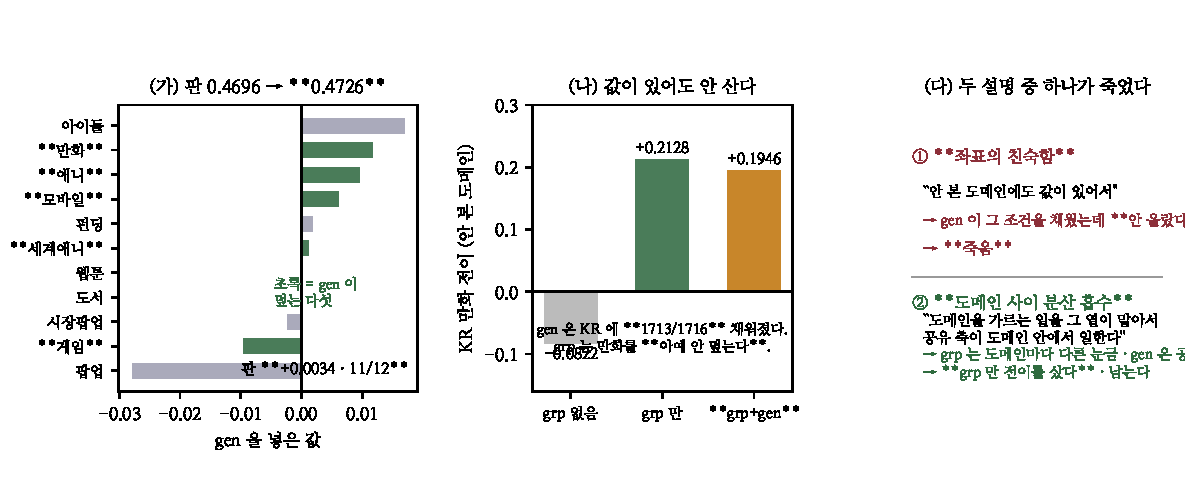
\includegraphics[width=\textwidth]{figs/fig419.pdf}
\caption{(가) gen 은 제가 덮는 도메인을 올린다. (나) 안 본 도메인에 값을
$1713/1716$ 채웠는데도 전이는 안 오른다. (다) 두 설명 중 ①이 죽는다.}
\end{figure}

\end{document}
